% -*- coding: utf-8 -*-
% !TEX root = ../main.tex

\subsection{Télécom SudParis}\label{ssec:introduction_nom_entreprise}

% TODO Présenter l'entreprise et ses objectifs
Télécom SudParis est une grande école d'ingénieurs du numérique localisée à Évry, en France, et certifiée par la Commission des Titres d'Ingénieurs.\
Celle-ci fait partie de l'Institut Mines-Télécom et est membre de l'Institut Polytechnique de Paris.\\
L'école compte environ 1000 étudiants et plus d'une centaine de doctorants.\
Les thématiques étudiées tournent autour des Mathématiques Appliquées, de l'Informatique, des Réseaux, du Signal, et de la Physique.\\
L'équipe pédagogique est composée de plus d'une centaine d'enseignants chercheurs dont les travaux portent sur des thématiques comme les
réseaux complexes, le big data, l'IA, le cloud, l'Internet des objets ou encore la cybersécurité.\

% Exemple pour pour une image
% Rappel | Formats acceptés par \includegraphics (défaut) : png, jpg, pdf...
\begin{figure}[!h]
    \centering
    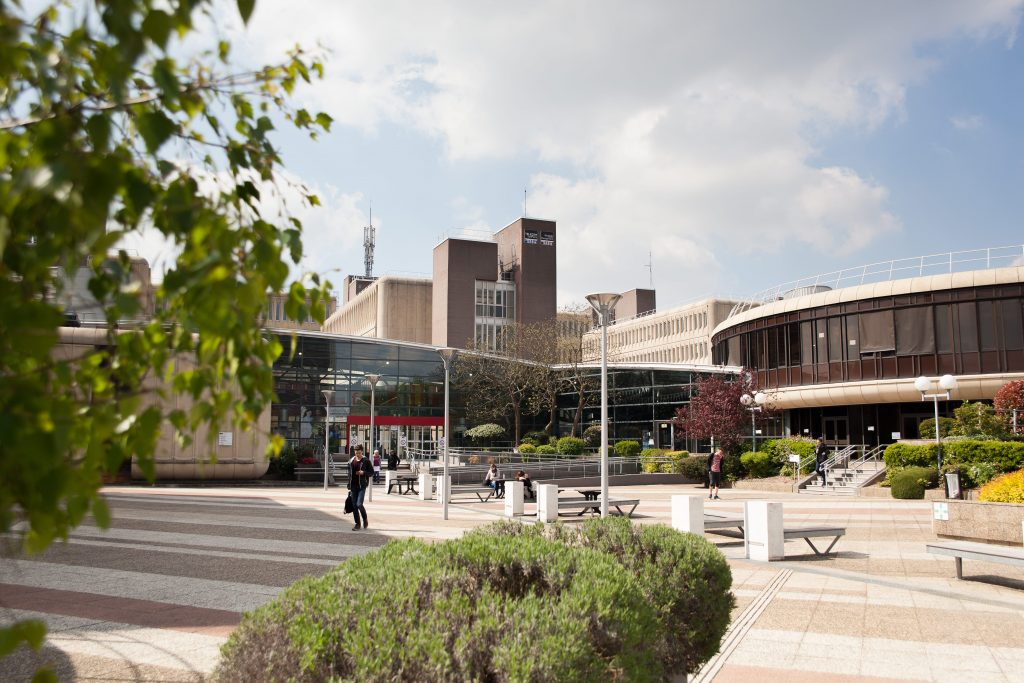
\includegraphics[width=0.7\textwidth]{img/campus_tsp.jpg}
    \caption{Photo du site}
    \label{fig:photo_site}
\end{figure}

%%%%%%%%%
%%%%%%%%%
%%%%%%%%%
%%%%%%%%%

\subsection{Service d'accueil}\label{ssec:introduction_service_accueil}

Ce stage a été encadré par \verb!François TRAHAY!, enseignant à \verb!Télécom SudParis! et chercheur au sein du laboratoire de recherche \verb!SAMOVAR! (Serivces répartis,\
Architectures, Modélisation, Validation, Administration des Réseux). Ce laboratoire accueille également quelques enseignants-chercheurs de l'\verb!ensIIE!, comme \verb!Valentin HONORÉ! qui a notamment co-encadré ce stage.\
Leurs travaux de recherche récents sont orientés vers l'analyse des performances dans le domaine du HPC (High Performance Computing).\
De plus, ils font partie de l'équipe \verb!BENAGIL! qui étudie la conception de systèmes distribués plus efficaces et plus sûrs en se focalisant sur leurs composants essentiels.

% TODO Présenter service/département de travail et son rôle dans entreprise
% On pourra aussi préciser le matériel à notre disposition pour mener notre stage

%%%%%%%%%
%%%%%%%%%
%%%%%%%%%
%%%%%%%%%

\subsection{Contexte et problématique}\label{ssec:introduction_contexte_problematique}

% TODO Présenter le contexte du stage et identifier les problèmes rencontrés qui justifient la pertinence du stage

%%%%%%%%%
%%%%%%%%%
%%%%%%%%%
%%%%%%%%%

\subsection{Objectifs du stage}\label{ssec:introduction_objectifs}

% TODO Présenter les objectifs du stage

%%%%%%%%%
%%%%%%%%%
%%%%%%%%%
%%%%%%%%%

\subsection{Contributions principales}\label{ssec:introduction_contributions}

% TODO Résumé des contributions majeures apportées
